\documentclass[10pt,portuguese]{article}
\usepackage[portuguese]{babel}

\usepackage{fourier}
\usepackage[bottom]{footmisc}

\usepackage[]{graphicx}
\usepackage[]{color}
\usepackage{xcolor}
\usepackage{alltt}
\usepackage{listings}
\usepackage[T1]{fontenc}
\usepackage[utf8]{inputenc}
\setlength{\parskip}{\smallskipamount}
\setlength{\parindent}{5ex}
\usepackage{indentfirst}
\usepackage{listings}
\usepackage{setspace}
\usepackage{hyperref}
\hypersetup{
    colorlinks=true,
    linkcolor=auburn,
    filecolor=magenta,      
    urlcolor=blue, urlsize=2em
}

% Set page margins
\usepackage[top=100pt,bottom=100pt,left=68pt,right=66pt]{geometry}

% Package used for placeholder text
\usepackage{lipsum}

% Prevents LaTeX from filling out a page to the bottom
\raggedbottom

\definecolor{javared}{rgb}{0.6,0,0} % for strings
\definecolor{javagreen}{rgb}{0.25,0.5,0.35} % comments
\definecolor{javapurple}{rgb}{0.5,0,0.35} % keywords
\definecolor{javadocblue}{rgb}{0.25,0.35,0.75} % javadoc

\lstset{language=Java,
basicstyle=\footnotesize\ttfamily,
keywordstyle=\color{javapurple}\bfseries,
stringstyle=\color{javared},
commentstyle=\color{javagreen},
morecomment=[s][\color{javadocblue}]{/**}{*/},
numbers=left,
numberstyle=\tiny\color{black},
stepnumber=2,
numbersep=10pt,
tabsize=4,
showspaces=false,
showstringspaces=false}


\usepackage{fancyhdr}
\fancyhf{} 
\fancyfoot[C]{\thepage}
\renewcommand{\headrulewidth}{0pt} 
\pagestyle{fancy}

\usepackage{titlesec}
\titleformat{\chapter}
   {\normalfont\LARGE\bfseries}{\thechapter.}{1em}{}
\titlespacing{\chapter}{0pt}{50pt}{2\baselineskip}

\usepackage{float}
\floatstyle{plaintop}
\restylefloat{table}

\usepackage[tableposition=top]{caption}


\definecolor{light-gray}{gray}{0.95}

\renewcommand{\contentsname}{Índice}

\begin{document}


\begin{titlepage}
	\clearpage\thispagestyle{empty}
	\centering
	\vspace{2cm}

	
	{\Large  Base de Dados \par}
	\vspace{0.5cm}
	{\small Carlos Costa\par
	Joaquim Sousa Pinto\par
	Sérgio Matos\par}
	\vspace{4cm}
	{ \textbf{Base de Dados de uma Perfumaria:}} \\
	\vspace{0.5cm}
	{\Huge \textbf{Perfumaria Orquídea}} \\
	\vspace{1cm}
	\vspace{4cm}
	{\normalsize  \par Pedro Bastos, 93150 \par Hugo Almeida, 93195
	   \par}
	 
	\vspace{2cm}

    
\includegraphics[scale=0.20]{logo_ua.png}
    
    \vspace{2cm}
    
	{\normalsize DETI \\ 
		Universidade de Aveiro \par}
		
	{\normalsize 12-06-2020 \par}
	\vspace{2cm}
		
	
	\pagebreak

\end{titlepage}
\tableofcontents{}
\clearpage

\section{Introdução}

\pa

\clearpage
\section{Análise de Requisitos}

\par Esta solução de base de dados está idealizada para ser implementada numa plataforma online de vendas de uma perfumaria que também tem um salão de estética. Após o processo de comunicação com o cliente da solução de base de dados, familiar de um membro do grupo, foi feita esta análise de requisitos.

\par \textbf{Informação associada ao “problema” do mundo:}
\par Existem \textbf{Utilizadores} na plataforma que podem ser do tipo Cliente ou Funcionário. Ambos têm os seguintes dados guardados, sendo que os a negrito são obrigatórios:

\begin{itemize}
    \item \textbf{Sexo}
    \item \textbf{Data de Nascimento}
    \item Morada
    \begin{itemize}
        \item Endereço
        \item Apt./Suite/Andar
        \item Localidade
        \item País
        \item Código-Postal
    \end{itemize}
    \item \textbf{Nome}
    \begin{itemize}
        \item \textbf{Primeiro Nome}
        \item \textbf{Último Nome}
     \end{itemize}
     \item \textbf{Email}
     \item \textbf{Password}
     \item Telemóvel
     \item Número Contribuinte
     \item Foto
\end{itemize}

\par Existem \textbf{Produtos} na plataforma que podem ser do tipo Perfume ou Cosmética. Ambos têm os seguintes dados guardados, sendo que os a negrito são obrigatórios:

\begin{itemize}
    \item \textbf{Imagem}
    \item \textbf{Identificador}
    \item Descrição
    \item \textbf{Marca}
     \item \textbf{Nome}
     \item Linha 
     \item Tamanho
     \item Categoria do utilizador - Homem/Senhora/Criança (Destinatário)
     \item \textbf{Categoria do Produto - After-Shave/Rosto}
     \item \textbf{Preço}
     \item Família Olfativa
\end{itemize}

\par Existem \textbf{Compras} na plataforma que podem ser do tipo Presencial ou Online. Ambos  têm os seguintes dados guardados, sendo que os a negrito são obrigatórios:

\begin{itemize}
    \item \textbf{Número de Compra}
    \item \textbf{Número de contribuinte do cliente}
    \item \textbf{Data da compra}
    \item \textbf{Tipo de Pagamento}
\end{itemize}

\par Existem \textbf{Cupões} na plataforma que podem ter os seguintes dados guardados, sendo que os a negrito são obrigatórios:

\begin{itemize}
    \item \textbf{Data de início da validade}
    \item \textbf{Data de final da validade}
    \item \textbf{Identificador}
    \item \textbf{Pontos que atribui}
\end{itemize}

\par Existem \textbf{Serviços} na plataforma que podem ter os seguintes dados guardados, sendo que os a negrito são obrigatórios:

\begin{itemize}
    \item \textbf{Tipo}
    \item \textbf{Identificador}
    \item \textbf{Preço}
    \item \textbf{Duração}
\end{itemize}

\par Existem utilizadores do tipo \textbf{Funcionários} na plataforma que podem ter os seguintes dados guardados, sendo que os a negrito são obrigatórios:

\begin{itemize}
    \item \textbf{Indicação se é Administrador}
    \item \textbf{Salário}
\end{itemize}

\clearpage

\par Existem utilizadores do tipo \textbf{Clientes} na plataforma podem ter os seguintes dados guardados, sendo que os a negrito são obrigatórios:

\begin{itemize}
    \item \textbf{Pontos}
    \item Forma de Pagamento
    \item \textbf{Indicação de subscrição de Newsletter}
\end{itemize}

\par Existem produtos do tipo \textbf{Cosmética} na plataforma podem ter os seguintes dados guardados, sendo que os a negrito são obrigatórios:


\begin{itemize}
    \item Tipo do produto - Desmaquilhantes/Tónicos…
\end{itemize}


\par Existem Compras do tipo \textbf{Online} na plataforma podem ter os seguintes dados guardados, sendo que os a negrito são obrigatórios:

\begin{itemize}
    \item Rating da encomenda por estrelas
    \item \textbf{Escolha se quer ser embrulhado como presente}
    \item \textbf{Morada}
    \begin{itemize}
        \item \textbf{Endereço}
        \item \textbf{Apt./Suite/Andar}
        \item \textbf{Localidade}
        \item \textbf{País}
        \item \textbf{Código-Postal}
    \end{itemize}
    \item \textbf{Telemóvel} 
    \item Observações
    \item Número de rastreio
\end{itemize}

\par Um cliente pode adicionar produtos como favoritos.
\par Um cliente pode usar um cupão uma única vez para adicionar pontos à sua conta.
\par Um cliente pode realizar várias compras quer estas sejam presenciais ou online. Por predefinição, os dados como Nº Contribuinte, Tipo de pagamento, Telemóvel (apenas compra online), etc, da compra são os dados que o utilizador tem guardado na sua conta, podendo ser guardados dados diferentes naquela compra em questão.
\par Nos dados de um cliente, tanto a morada como o tipo de pagamento, telemóvel e número de contribuinte são opcionais sendo que ao realizar uma compra, muitos destes são definidos para a compra em questão e poderão (ou não) ser guardados na tabela do utilizador.
\par Um produto pode ter uma promoção associada com o respectivo nome e percentagem de desconto.
\par Ao realizar uma compra, esta compra vai ser composta por produtos com as respetivas unidades adquiridas. Na compra podem ser descontados os pontos do cliente e/ou acumulados.
\par Um cliente pode marcar um serviço, ficando a data dessa marcação guardada.
\par A duração do serviço depende do funcionário que o realiza.
Uma compra presencial tem obrigatoriamente um funcionário a supervisionar.

\clearpage

\section{DER}

\begin{figure}[!h]
    \centering
    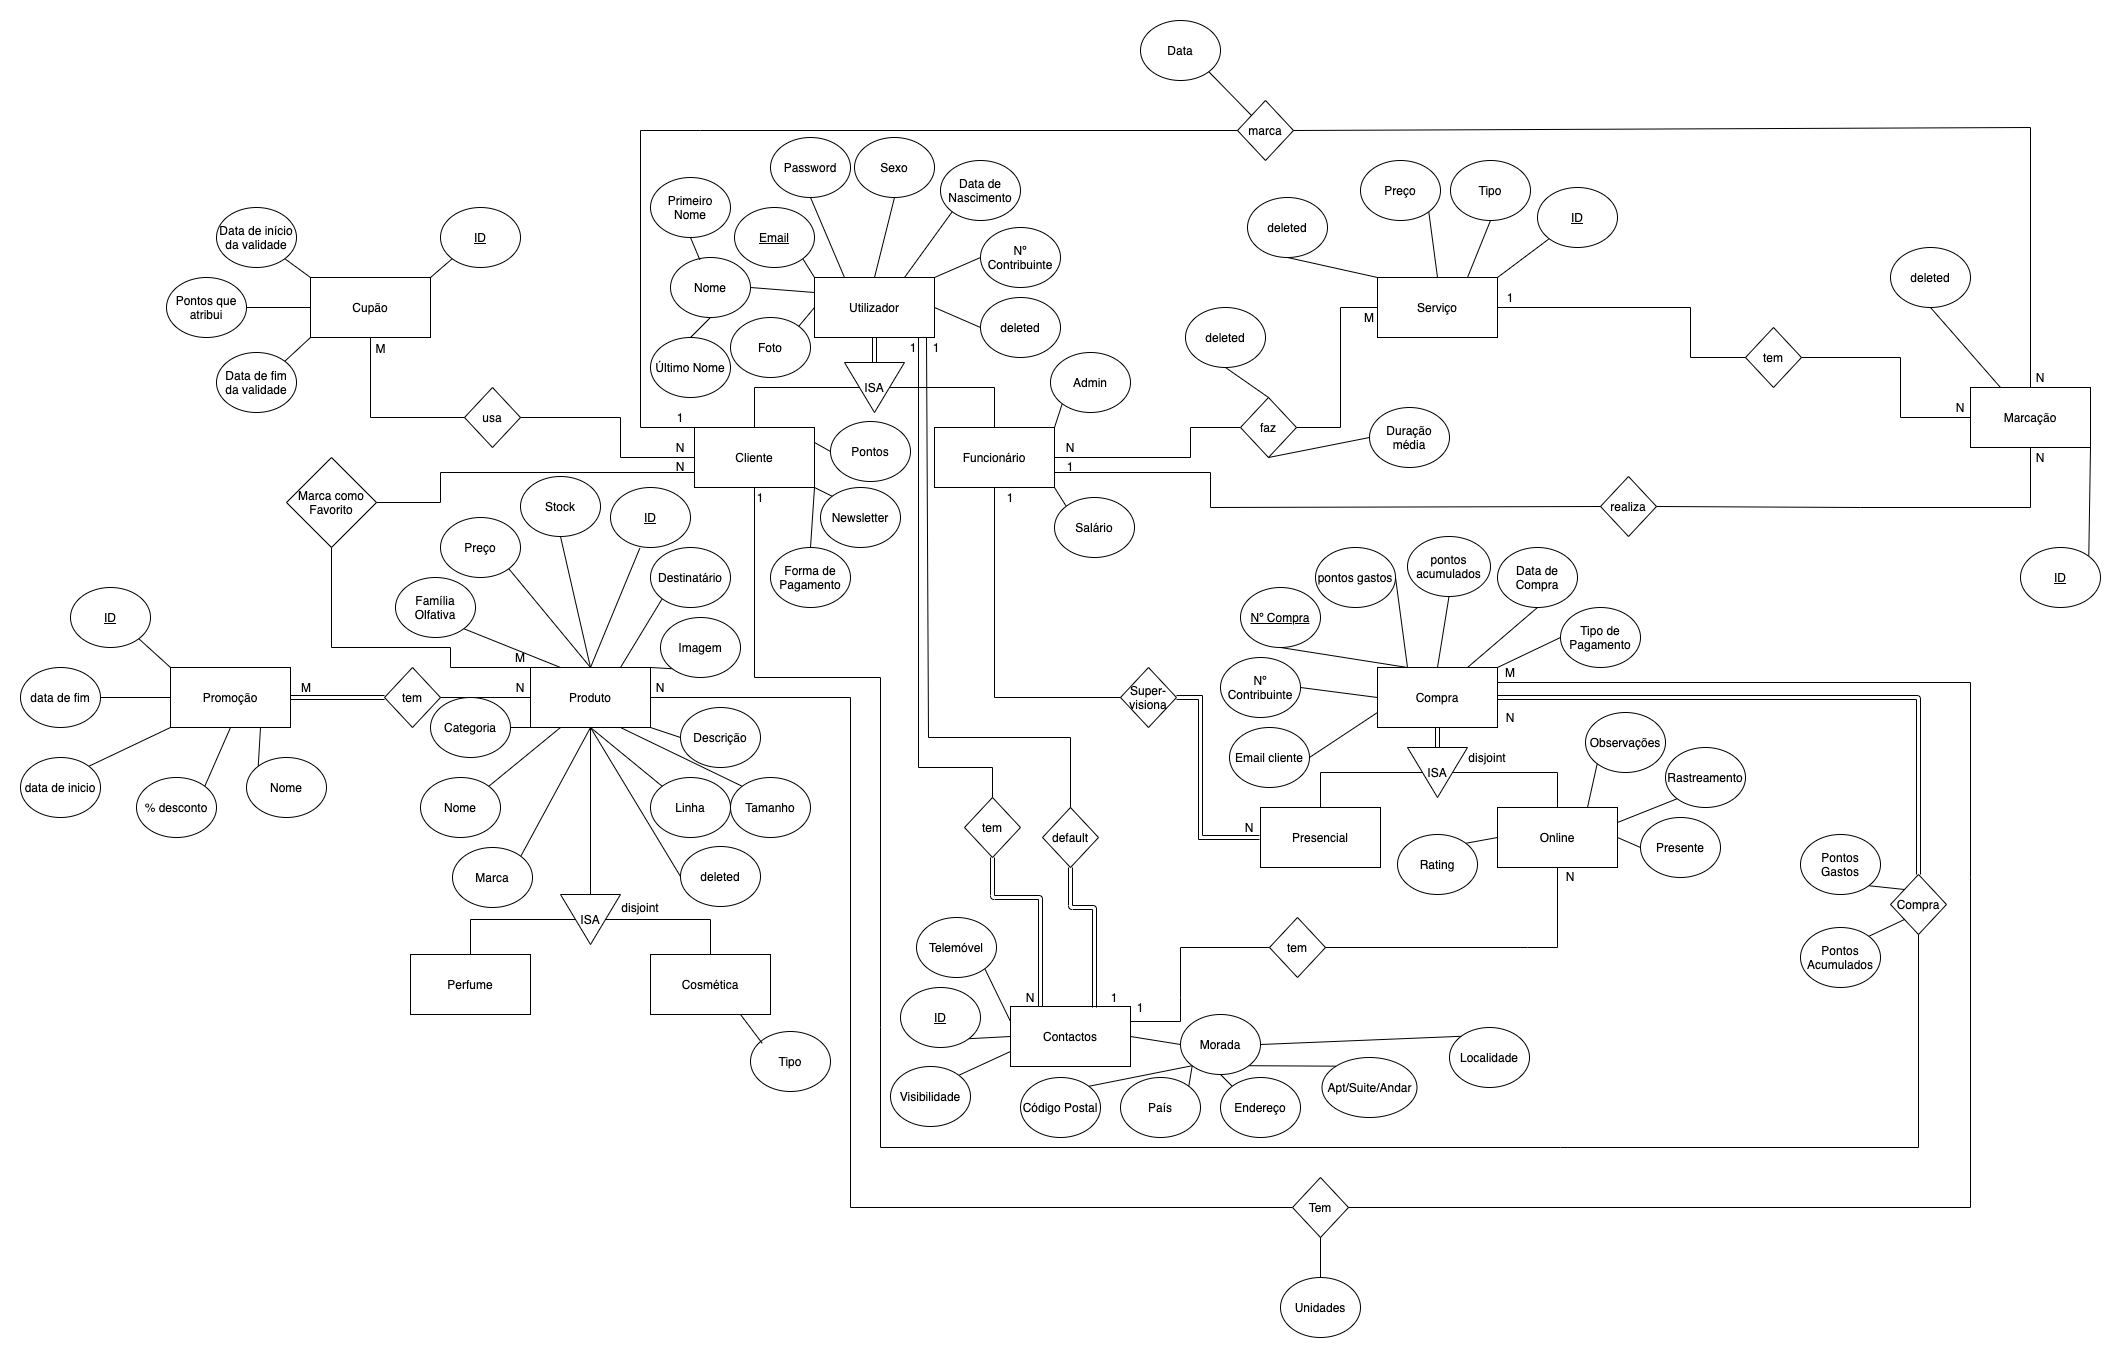
\includegraphics[width=\textwidth]{images/DER.png}
    \caption{Diagrama Entidade/Relação da proposta de base de dados apresentada pelo grupo}
\end{figure}

\clearpage

\section{Esquema Relacional da BD}

\begin{figure}[!h]
    \centering
    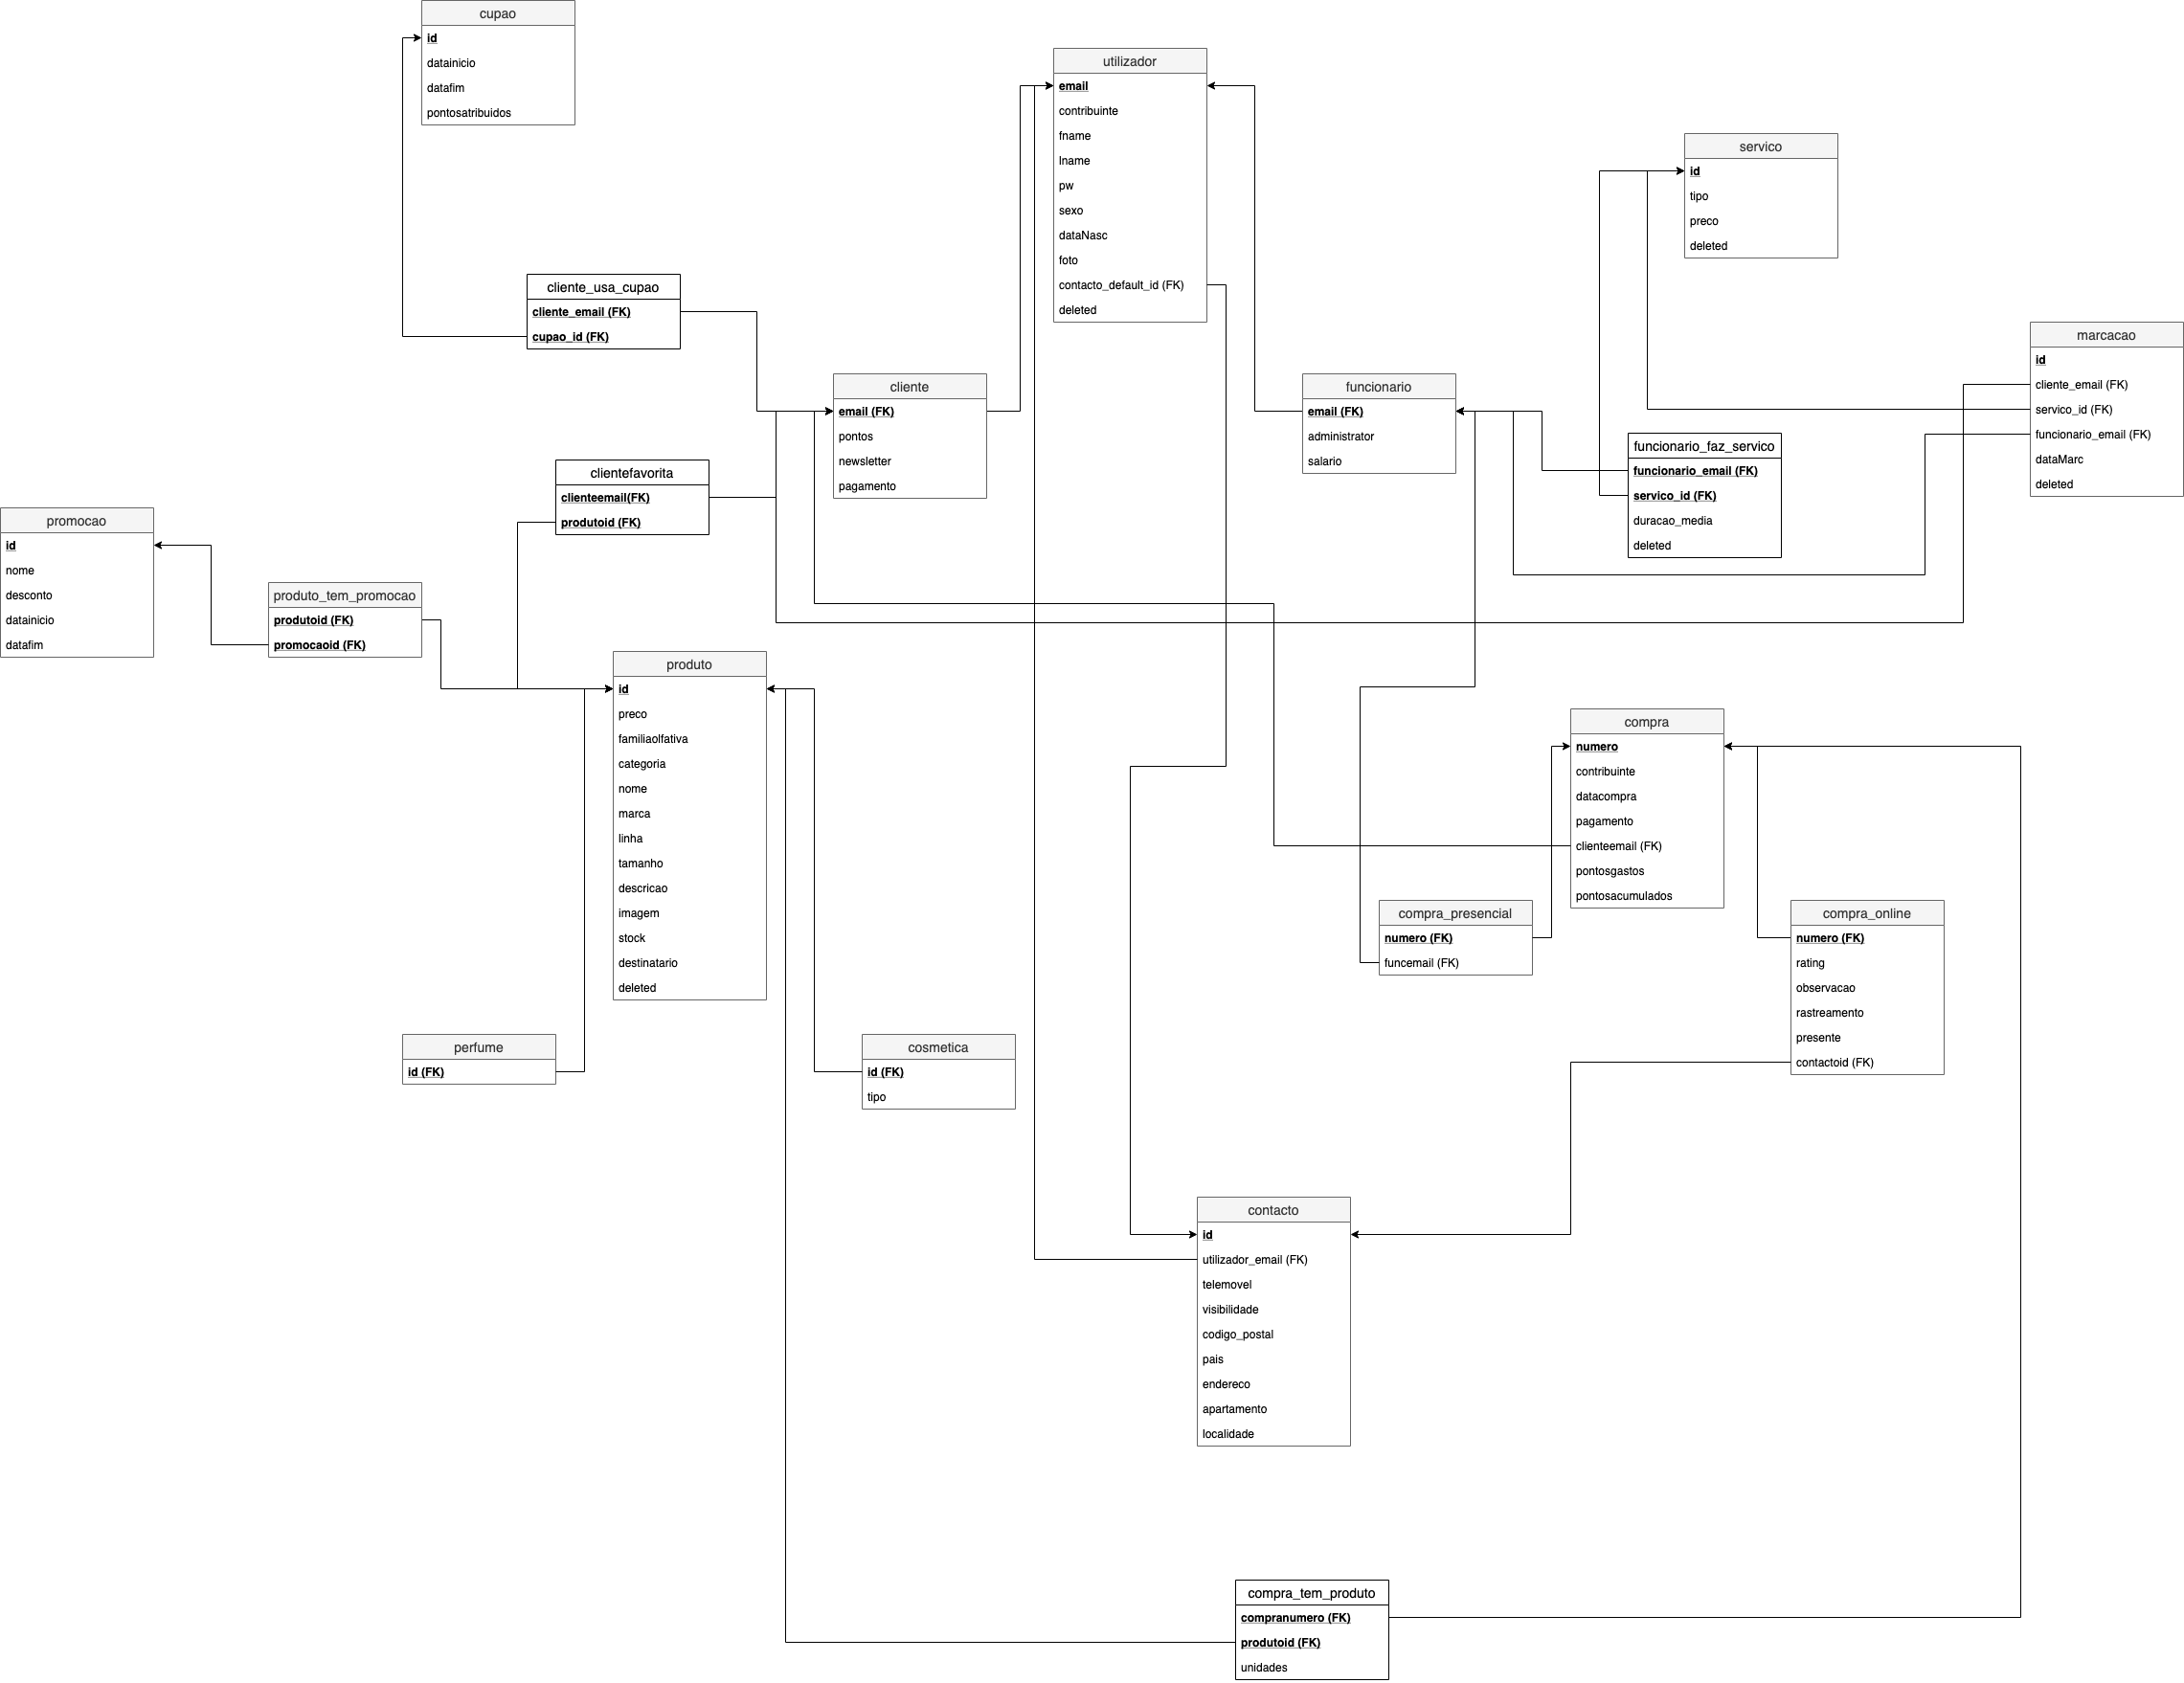
\includegraphics[width=\textwidth]{images/ER.png}
    \caption{Modelo Entidade/Relação da proposta de base de dados apresentada pelo grupo}
\end{figure}

\clearpage

\section{SQL DDL}

\par Foi criada uma Base de dados local com o nome de "Perfumaria" e posteriormente criado o \textit{Schema} \textit{"perf"}. Assim, as tabelas têm como nome "Perfumaria.perf.[TableName]".

\begin{figure}[!h]
    \centering
    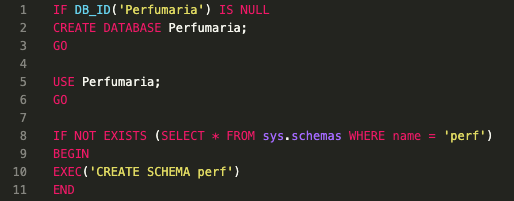
\includegraphics[width=300]{images/DDL_BD.png}
    \caption{Criação da Base de dados e Schema}
\end{figure}

\par A criação das tabelas é sempre feita da mesma forma, como visível na Figura 4. A tabela \textit{Perfumaria.perf.utilizador} tem a particularidade de, por questões de segurança, apenas guardar o valor do \textit{Hash} da password que o utilizador coloca (criado através de um \textit{Stored Procedure}). Assim, a password nunca chega a ser guardada na BD, apenas é guardado o \textit{Hash}. 

\begin{figure}[!h]
    \centering
    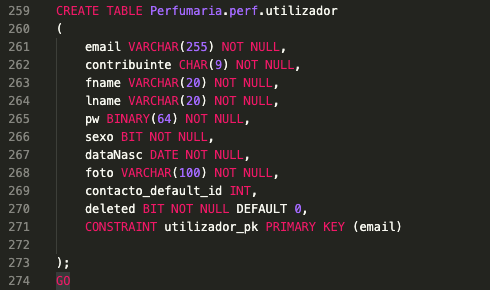
\includegraphics[width=300]{images/utilizador.png}
    \caption{Tabela Perfumaria.perf.utilizador}
\end{figure}

\par As \textit{Foreign Keys} são adicionadas no fim do \textit{script} para evitar conflitos, sendo que existem verificações iniciais para, se necessário, ser feito o \textit{Drop} de \textit{Constraints}.

\clearpage

\section{SQL DML}

\par Todos os comandos de \textit{SQL DML} foram executados dentro de \textit{Stored Procedures, UDFs e Triggers} de maneira a criar uma camada de abstração entre a interface e a Base de Dados, aumentando a segurança com uma série de verificações, evitando \textit{SQL Injections} e permitindo o encapsulamento da mesma.

\section{Normalização}
\par Tendo em conta o objetivo do processo de desenho de uma base de dados relacional relativamente a minimizar a redundância dos dados, foram feitos diversos testes para verificar que formas normais esta respeitava (processo de normalização).

\par Após estas verificações, foi concluído que o modelo de dados se encontrava na Terceira Forma Normal (\textit{3FN}), respeitando também as formas normais anteriores. Com isto em consideração, concluiu-se que as relações estavam normalizadas, não necessitando quando tipo de alterações.

\section{Índices}

\par Ao analisar o tipo de \textit{queries} feitas pela aplicação e qual a sua frequência, foi concluído que faria sentido utilizar um índice composto \textit{Non-clustered} para melhorar a performance das pesquisas e filtros da visualização dos produtos. Dito isto, foi criado o \textbf{índice composto \textit{Non-clustered} (preco, marca, nome, categoria)} da tabela \textbf{produto}, permitindo melhoria da performance a \textit{queries} que incluam filtros ou pesquisas com:
\begin{itemize}
    \item Preço 
    \item Preço e Marca
    \item Preço, Marca e Categoria
    \item Preço, Marca, Nome e Categoria
\end{itemize}

\par É expectável a utilização destes filtros, especialmente com preço, pois os produtos são carregados inicialmente na aplicação ordenados pelo preço. Futuramente com a utilização da aplicação por utilizadores, faria sentido verificar se o restante das presunções se mantêm no entanto, nos testes que foram feitos à performance da \textit{queries} antes e depois da utilização do índice, ao utilizá-lo, o \textit{Estimated Subtree Cost} foi inferior.

\par Por outro lado, não foram utilizados outros índices pelo simples facto que maior parte das restantes \textit{queries} lidam com as entidades através de pesquisa com as \textit{Primary Keys} que, por si só, já são por \textit{default} um índice \textit{Clustered}.

\clearpage

\section{Triggers}

\par Foram criados \textit{Triggers After} para automaticamente serem executadas ações e algumas verificações após determinadas chamadas \textit{DML}, com o objetivo de manter a integridade dos dados.

\par Um dos quatro exemplos utilizados é a adição de pontos à conta do cliente após a utilização de um cupão (validado anteriormente através de um \textit{Stored Procedure}):

\begin{figure}[!h]
    \centering
    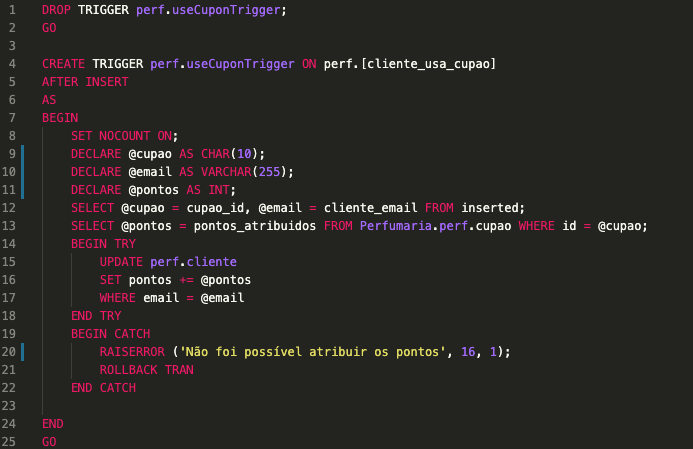
\includegraphics[width=410]{images/useCuponTrigger.png}
    \caption{\textit{Trigger After Insert} de um cupão na tabela \textit{cliente\_usa\_cupao}}
\end{figure}

\par Os outros 3 \textit{Triggers After}, \textit{buyProduct}, \textit{changeProduct} e \textit{createContact} verificam se os produtos necessitam de passar para eliminados (através do atributo \textit{deleted}) consoante o \textit{stock} ou, se o utilizador passa a ter um contacto como \textit{default}, após a sua criação, se ainda não tiver nenhum.

\par Foi escolhido o uso de \textit{Stored Procedures} ao invés de \textit{Triggers Instead Of} para verificações antes da execução de chamadas \textit{DML} pois, a aplicação utiliza-os sempre para fazer alterações de dados e nunca foi necessária a substituição de uma chamada por outra.

\clearpage

\section{Stored Procedures}

\par Com foi referido anteriormente, grande parte das chamadas à BD são feitas através de Stored Procedures, criando assim a camada de abstração. Resumindo, foram criadas SPs para adicionar elementos às tabelas, como por exemplo addContact, addCupon, addFuncService, addMarc, etc.

\begin{figure}[!h]
    \centering
    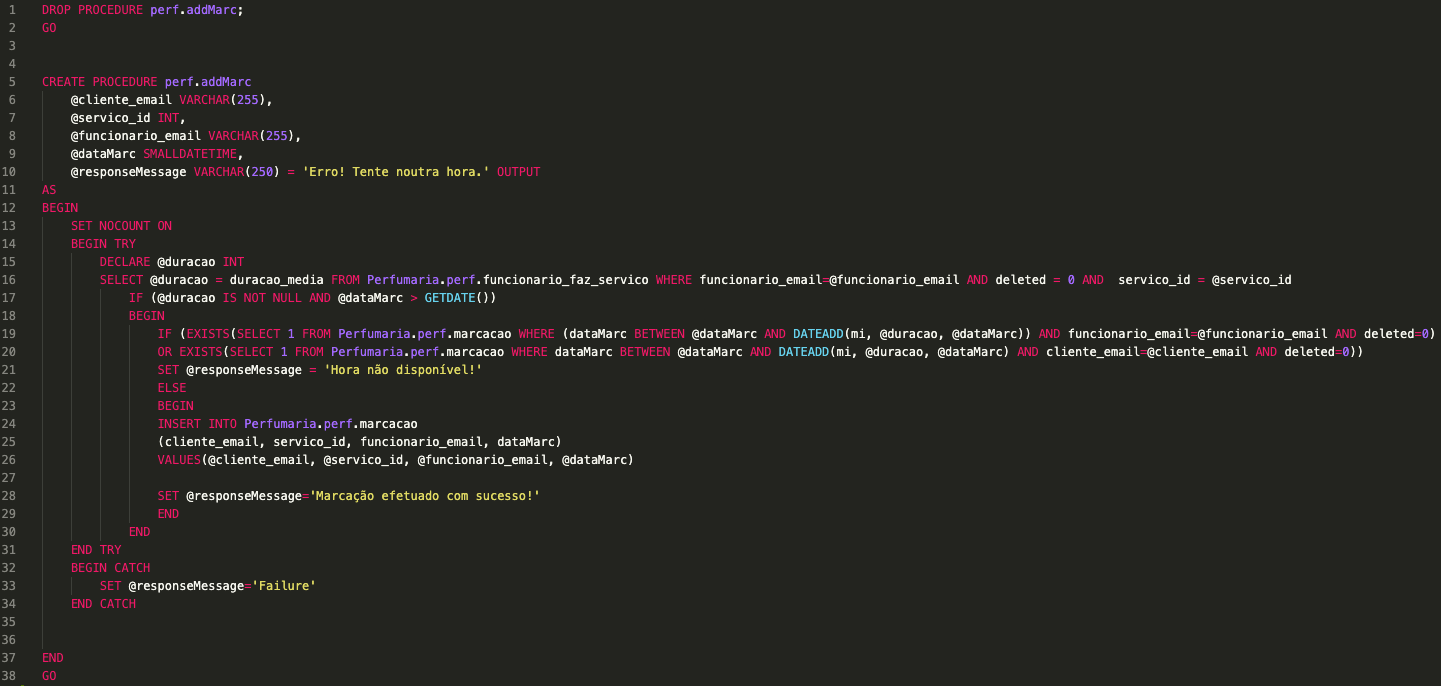
\includegraphics[width=410]{images/addMarc.png}
    \caption{Exemplo de uma Stored Procedure de adição}
\end{figure}


\par Foram também criadas SPs para alterar valores de uma tabela, como por exemplo changeDefaultContact, changeProduct, updateFunc, updateMarc, etc.

\begin{figure}[!h]
    \centering
    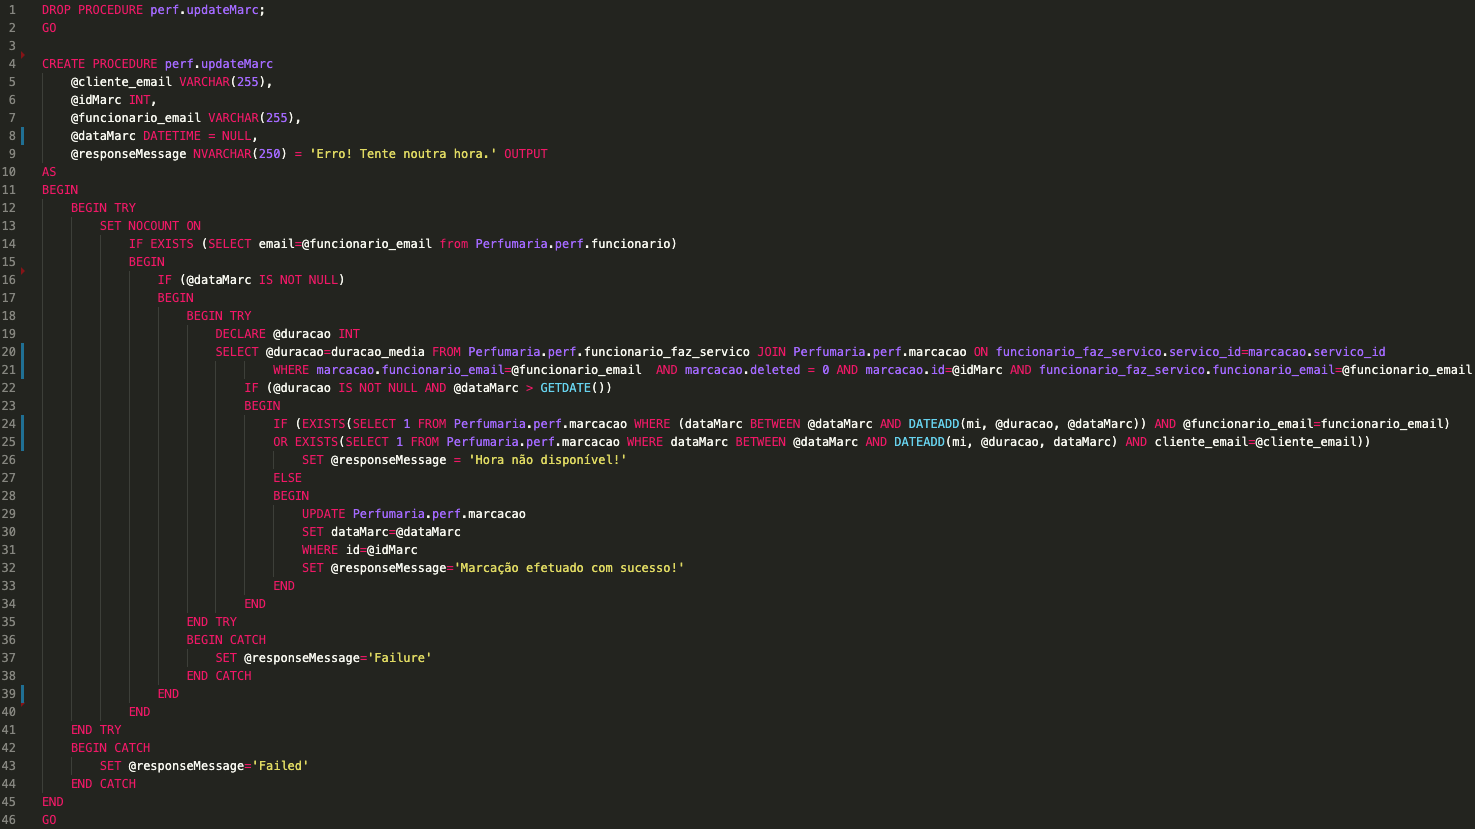
\includegraphics[width=410]{images/updateMarc.png}
    \caption{Exemplo de uma Stored Procedure de update}
\end{figure}

\par Tem também alguns gets mais complexos, como por exemplo o getDetailsFromBuy, getDetailsFromSell, getProductFilters, etc.

\begin{figure}[!h]
    \centering
    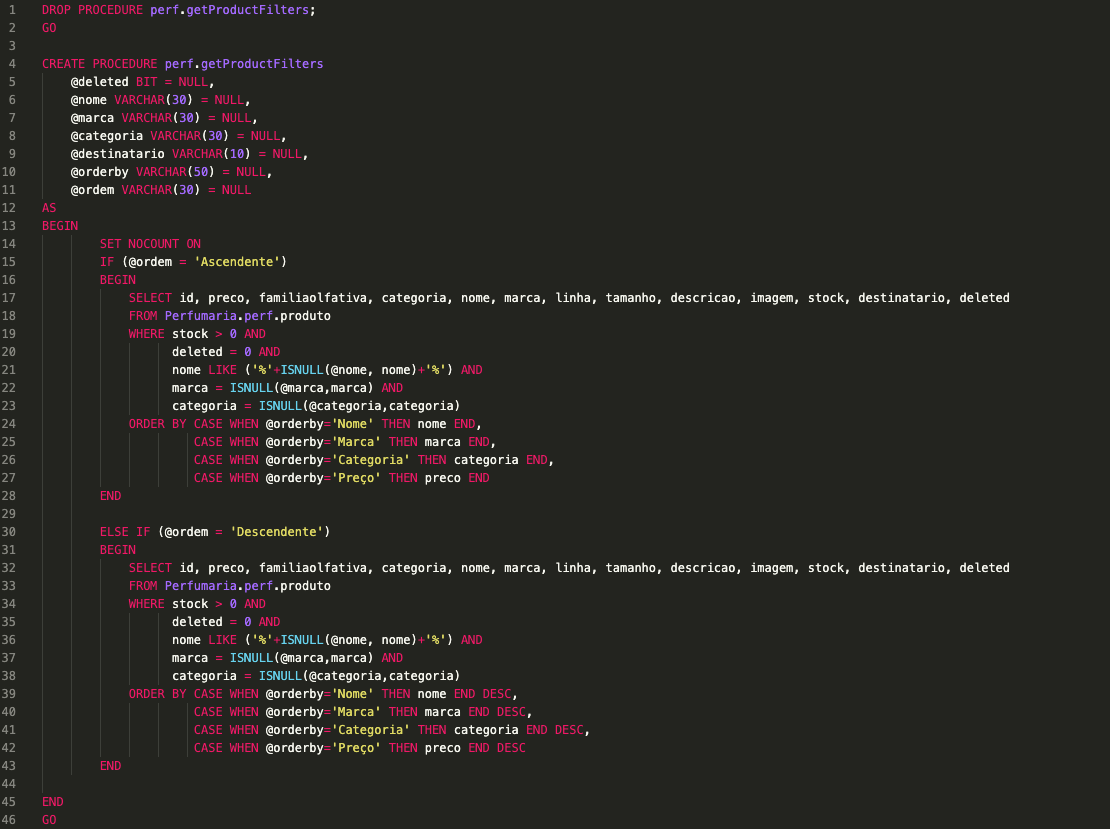
\includegraphics[width=500]{images/getProductFilters.png}
    \caption{Exemplo de uma Stored Procedure de um get}
\end{figure}

\clearpage

\par Finalmente, tem algumas SPs para ações mais específicas. Dentro destas, as mais importantes são login, registerFunc e registerClient, que permitem o sistema de login inicial da nossa BD.

\begin{figure}[!h]
    \centering
    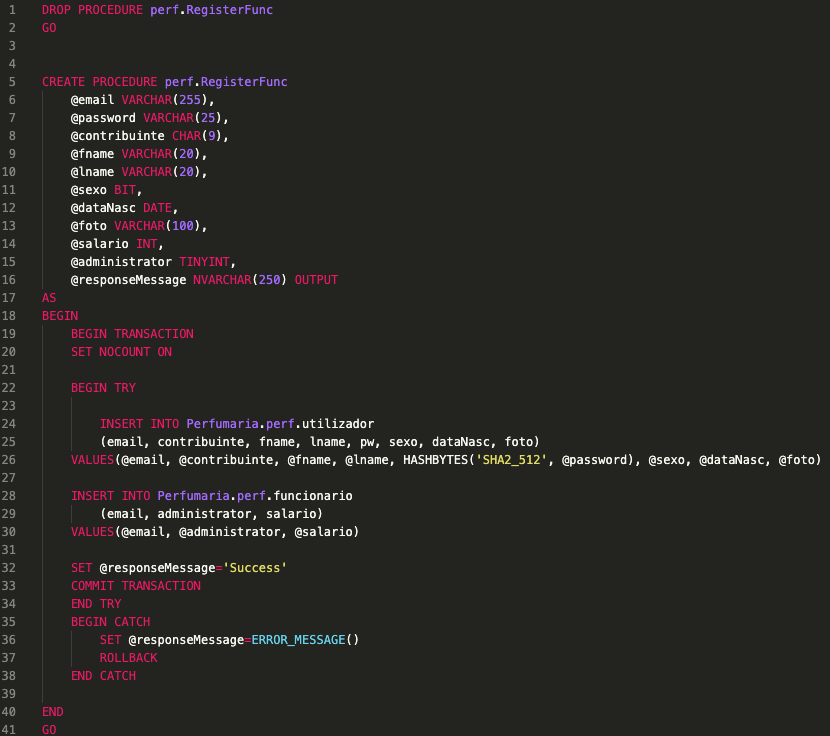
\includegraphics[width=\textwidth]{images/registerFunc.png}
    \caption{SP de Registo de um funcionário}
\end{figure}


\clearpage

\section{UDF}

\par Foram também utilizadas UDFs para a execução de queries mais simples, isto é, para apenas ir buscar valores de certas tabelas. Usamos UDFs Inline Table-Valued, como por exemplo clientBuyHistory, funcFutureMarc, etc.

\begin{figure}[!h]
    \centering
    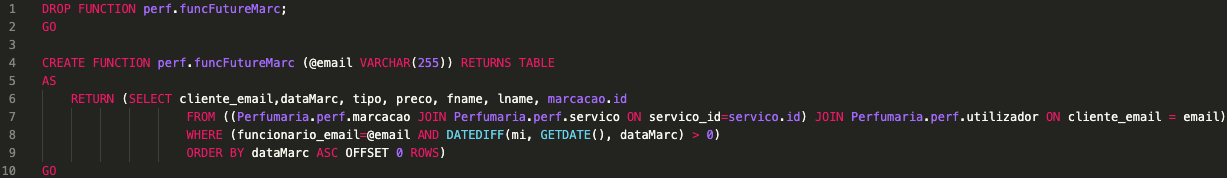
\includegraphics[width=\textwidth]{images/funcFutureMarc.png}
    \caption{Exemplo de UDF Inline Table-Valued}
\end{figure}

\par Alem das Inline, utilizamos também as Multi-Statement Table-Valued para queries simples mas que necessitavam de verificações iniciais, como por exemplo getAllFuncs, getAllProducts, etc.

\begin{figure}[!h]
    \centering
    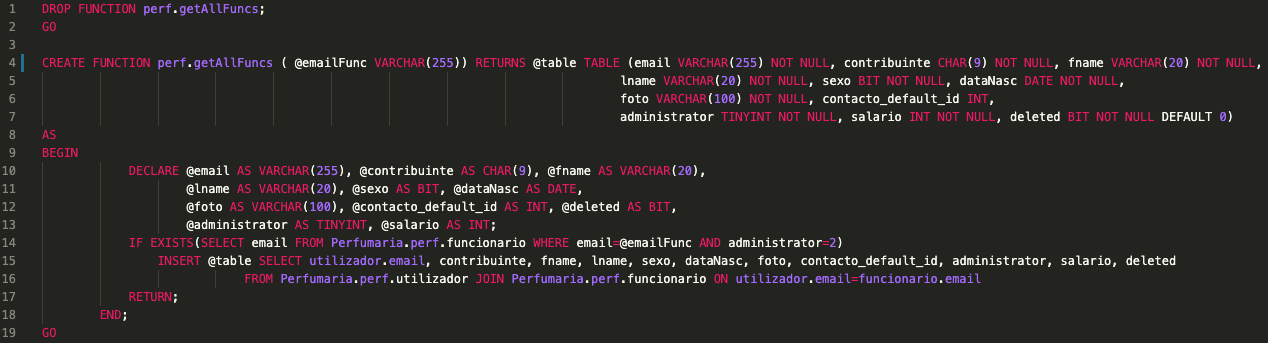
\includegraphics[width=\textwidth]{images/getAllFuncs.png}
    \caption{Exemplo de UDF Multi-Statement Table-Valued}
\end{figure}

\clearpage

\section{Transações}

\par Para garantir a consistência dos dados, foram utilizadas Transações que, com a sua atomicidade, garantem que, mesmo que uma das execuções de modificações de dados falhem, as outras todas são revertidas, mantendo coerência e integridade na Base de Dados. Estas foram utilizadas em casos onde existem múltiplas modificações de dados num \textit{script} e é necessário garantir a sua execução total.

\begin{figure}[!h]
    \centering
    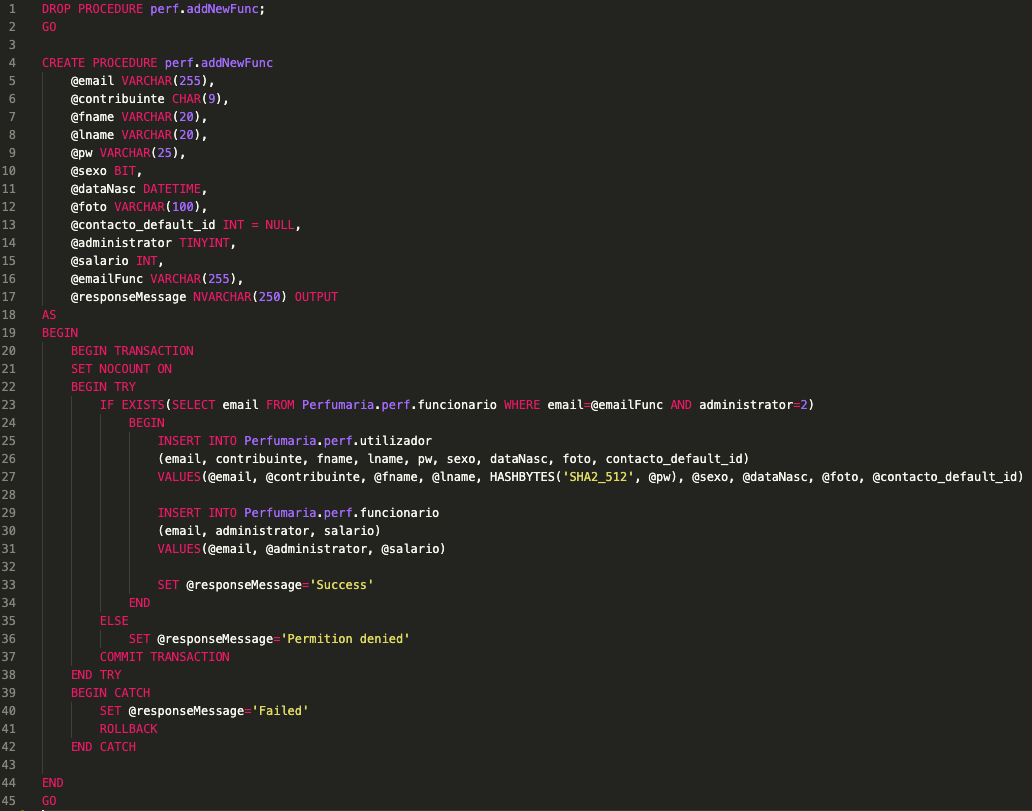
\includegraphics[width=410]{images/addNewFunc.png}
    \caption{Exemplo de uma Transação, mantendo a consistência dos dados}
\end{figure}

\section{Conclusão}

\clearpage

\section{Bibliografia}

\bibliographystyle{plain}

\bibliography{biblist}

\vspace{5mm} %5mm vertical space

[1] Material fornecido pelo Docente de Base de Dados



\end{document}

